% ==============================================================================================
\chapter{Dynamic horizontal point load on dam} \label{ch:vibrating_dam}
% ==============================================================================================

% ----------------------------------------------------------------------------------------------
\section{Introduction}
% ----------------------------------------------------------------------------------------------
This benchmark compares the STEM numerical solution against an analytical solution for the natural frequencies of a
dam subjected to a dynamic horizontal point load under plane-strain conditions.

The analytical solution is presented in~\cite{Kramer_1996}. The analytical solution provides the first
5 natural frequencies of vibration of the dam structure, which are compared against the numerical model.

% ----------------------------------------------------------------------------------------------
\section{Model Description}
% ----------------------------------------------------------------------------------------------

% ..............................................................................................
\subsection{Geometry, mesh and loading}
% ..............................................................................................
The reference geometry as presented in~\cite{Kramer_1996} is given with feet units. For consistency with the rest of
the benchmarks in this report, the geometry has been converted to SI units (meters).

The analytical solution is formulated in plane-strain conditions. To mimic this, two analyses are performed:
a two-dimensional analysis representing a dam in plane-strain conditions, and a three-dimensional
analysis representing a dam in a full 3D setting, where the thickness in the out-of-plane direction is set to
\qty{1}{\meter} and the displacements are fixed in the out-of-plane direction. This allows to verify that the
three-dimensional solution converges to the analytical solution.

In the two-dimensional analysis, the soil domain is modelled as a
triangle with base \qty{160.02}{\meter} and height \qty{45.72}{\meter},
the left slope is inclined with a ratio of 2:1 (horizontal to vertical), while the right slope is inclined with a ratio
of 1.5:1. The mesh is created with second-order triangular elements and uses an average element size of \qty{2}{\meter}.

In the three-dimensional analysis, the soil domain is modelled as a triangular prism with base
\qty{160.02}{\meter} and height \qty{45.72}{\meter},
the left slope is inclined with a ratio of 2:1 (horizontal to vertical), while the right slope is inclined with a ratio
of 1.5:1. The geometry is extruded to \qty{4}{\meter} thickness in the z-direction to create a 3D model.
The mesh is created with second-order tetrahedron elements and uses an average element size of \qty{2}{\meter}.

Figure~\ref{fig:vibrating_dam_mesh_3d} illustrates the geometry and mesh adopted for the analysis.

The horizontal load with a magnitude of \qty{1e6}{\newton\per\meter} is instantly applied at the top of the dam
structure and is kept constant during the analysed time window.
All nodes along the bottom boundary are fully fixed, while all remaining nodes are constrained to
move only in the horizontal x direction.


\begin{figure}
    \centering
    \begin{subfigure}[t]{0.49\textwidth}
        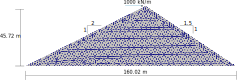
\includegraphics[width=0.75\textwidth]{vibrating_dam/vibrating_dam_mesh.pdf}
    \caption{}
    \label{fig:vibrating_dam_mesh_a}
    \end{subfigure}
    \begin{subfigure}[t]{0.49\textwidth}
        \includegraphics[width=0.75\textwidth]{vibrating_dam/vibrating_dam_mesh_3D.pdf}
    \caption{}
    \label{fig:vibrating_dam_mesh_b}
    \end{subfigure}
    \caption{Geometry and mesh for the vibrating dam benchmark in: (a) two-dimensional
     and (b) three-dimensional.}
    \label{fig:vibrating_dam_mesh_3d}
\end{figure}


% ..............................................................................................
\subsection{Materials and numerical parameters}
% ..............................................................................................
The soil is modelled as a one-phase continuum with a linear elastic constitutive law, with the
following parameters:

\begin{itemize}[noitemsep,topsep=0pt,parsep=0pt,partopsep=0pt]
    \item Young's modulus: \qty{722}{\mega\pascal},
    \item Poisson ratio: 0.49,
    \item Density: \qty{2000}{\kilogram\per\meter\cubed}.
\end{itemize}

Material damping is excluded from this analysis.

The dynamic analysis is performed over a \qty{2}{\second} time window, with a time step of \qty{0.001}{\second}.
The system of equations is solved using the Newmark time integration~\cite{Newmark_1959} scheme with
parameters $\beta = 0.25$ and $\gamma = 0.5$.

% ----------------------------------------------------------------------------------------------
\section{Results}
% ----------------------------------------------------------------------------------------------
Figure~\ref{fig:vibrating_dam_results} presents the power spectral density of the horizontal displacement of the
top of the dam.
The figure compares the STEM results against the analytical solution.
The peaks of the power spectral density occur at the expected first five natural frequencies,
showing an agreement between the numerical and analytical solutions.

\begin{figure}[h]
    \centering
    \includegraphics[width=0.8\textwidth]{vibrating_dam/power_spectral_density.pdf}
    \caption{Power spectral density plot of the horizontal displacement at the top of the dam}
    \label{fig:vibrating_dam_results}
\end{figure}
